\subsection{\texorpdfstring{W+jets Background Estimation in $\tauTau$ Channel}{W+jets Background Estimation in tau-tau Channel}}
\subsubsection{Method Description}
As shown in Table~\ref{tbl:cutflowtable}, the number of W+jets events surviving 
the selection cuts are found to be zero in search \binone or 0.43$\pm$0.40 in search \bintwo. 
Therefor, the statistical uncertainties on the expected yields of W+jets events
are huge, e.g. it reaches to 93\% in \bintwo. 
 The statistical uncertainty on the yields for W+jets events can be improved by extracting 
the $\mttwo$ or $\SumMT$ cut efficieny, depending on the serach bins, in a sample with more 
statistics. To make this sample, some cuts with small effects on the search variables are 
relaxed. Various samples with different relaxed cuts are examined to check the idea of small correlation 
between search variable and relaxed cuts. In the next section, the validation of this method will be discussed.\\
When the cut efficiency for the $\mttwo$ or $\SumMT$ variable is found, then it is multiplied by the W+jets 
yields before cutting on the search variable. This means, according to Table~\ref{tbl:cutflowtable}, the cut efficiency for 
$\mttwo$ ($\SumMT$) found in a relaxed sample should be multiplied by 31.93(29.13) to get an 
estimate for the W+jets events in search \binone (search \bintwo).\\
The systematics that can be assigned to this method is the maximum
variation of the estimations among those relaxed samples.
\subsubsection{Method Validation}
\begin{figure}[htbp]
\centering
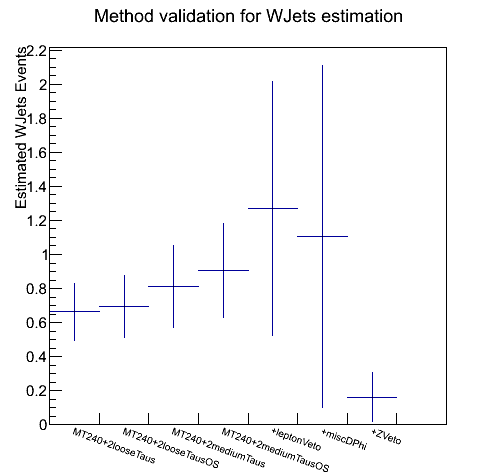
\includegraphics[angle=0,scale=0.35]{TauTauFigs/withMT2GT40.png}
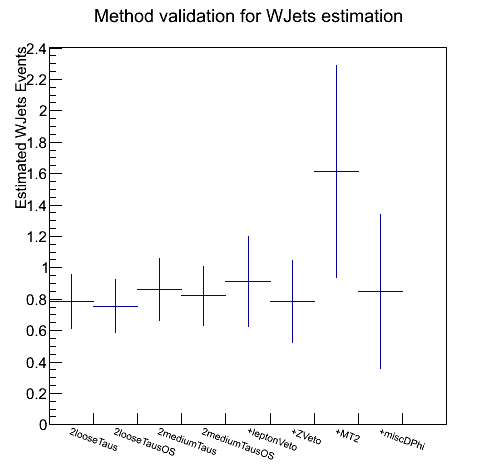
\includegraphics[angle=0,scale=0.35]{TauTauFigs/WJetsEst_bin2_BJetVetoApplied.png} \\
\caption{Cut efficiency for $\mttwo$ (\SumMT) (right) 
in samples with various selections as labeled in each bin.}
\label{fig:justification}
\end{figure}
Various samples with different relaxed cuts are used to estimate W+jets events. The estimated values 
for W+jets in search \binone (search \bintwo) in each sample is shown in the left (right) plot 
in Figure~\ref{fig:justification}. The list of cuts is given as the bin labels of the histograms. To be clear, e.g., 
the list of cuts for relaxed samples used in search \binone is as follows   
\begin{itemize}
\item only two loose hadronic taus are required;
\item only two OS loose hadronic taus are required;
\item only two medium hadronic taus are required;
\item only two OS medium hadronic taus are required;
\item on top of requiring two OS medium hadronic taus, extra lepton veto is applied;
\item in addition to the last mentioned set of cuts, $\mindphifour$ cut is applied;
\item Z veto is added to the list of previously mentioned set of cuts;
 \end{itemize}
As seen from Figure~\ref{fig:justification}, by adding more and more cuts, we are getting closer to the signal selection region 
and the cut efficiency of the search variable (or equivalently the estimated values for the search bin) 
appears with larger uncertainties. Overally the estimated values show a linear behavior and can be fit with a $pol0$ function. 
Therefore, not only these plots can be used to verify the method, but also show the final estimated W+jets events. We take the estimated 
values and corresponding statistical uncertainties from the first bin of the two plots. For the systematical uncertainty, we take the
difference between estimated values in the first and forth bin.\\
A summary of the estimated W+jets events can be found in Table~\ref{tbl:wjetsEstimation}. 


